\documentclass[12pt]{report}
\usepackage[utf8]{inputenc}
\usepackage{graphicx}
\usepackage[tmargin=2cm, lmargin=4cm, rmargin=2.5cm, bmargin=4cm, paperwidth=8.267in, paperheight=11.692in]{geometry}
\usepackage{amsfonts}
\usepackage{array}
\usepackage{indentfirst}
\graphicspath{ {images/} }
\usepackage{lipsum}
\usepackage{verbatim}
\usepackage{titlepic}
\usepackage{amsmath}
\usepackage{titlesec}

\begin{document}

\title{Wind Flow Sampling \linebreak Using an Autonomous UAV \vspace{2.5cm}}	%\includegraphics[scale=0.2]{university_edinburgh.jpg}
\titlepic{\includegraphics[scale = 0.55]{university_edinburgh.jpg}}
\author{
\Large Carson Vogt \vspace{1cm} \\ 
Supervisor: Subramanian Ramamoorthy \vspace{3cm}
}

\date{
	\centering
	Master of Science by Research \endgraf\medskip
	The University of Edinburgh \endgraf\medskip
	31 August 2015
}

\begin{comment}
\begin{figure}
\centering
\begin{minipage}{0.45\textwidth}
\centering
\includegraphics[scale=0.2]{university_edinburgh.jpg}
\end{minipage}\hfill
\begin{minipage}{0.45\textwidth}
\centering
\includegraphics[scale=0.2]{rad.jpg}
\end{minipage}
\end{figure}
%\begin{figure}[b]\begin{flushright}\includegraphics[scale=0.5]{rad.jpg}\end{flushright}
%\begin{flushleft}\includegraphics[scale=0.5]{university_edinburgh.jpg}\end{flushleft}
%\end{figure}
\end{comment}

\maketitle
%...will work on the images

\begin{abstract}
\begin{small}
Most unmanned aerial vehicles (UAVs) used today are employed for photography, search and rescue, or infrastructure monitoring, such as with pipelines or agriculture. However, relatively little attention has been paid to the medium in which the UAV operates: the atmosphere.
This work presents a novel system designed to utilize autonomous UAVs as a measurement tool, employing machine learning techniques and relying on atmospheric readings to reconstruct, interpolate, and regress the vector field through which it has flown. A week long experiment shows that such techniques can yield a full 2D wind map from sparse measurements, landscape features from wind pattern, and generate estimates from a model based on the experiment. The work shows potential application in weather prediction and infrastructure optimization for wind farms. The focus of the work is on the system as a whole, from the platform that was tediously tuned, printed, and assembled, to the algorithms on which the results are based. Future work regarding project developments and potential applications are covered at the end of the paper.
\end{small}
\end{abstract}

\chapter*{Declaration}
\vspace{3cm}
This thesis has been composed by Carson Vogt and is the sole work of the author. Sources and quotes have been acknowledged, with a bibliography listing all sources at the end. This work has not been submitted for any other degree or professional qualification.

\vspace{5cm}

Signature\hspace{2cm} \line(1,0){230}

\vspace{2cm}

Date\hspace{3cm}\line(1,0){230}

\listoffigures

\tableofcontents

\chapter{Introduction}
\section{Introduction}
Unmanned verial vehicles, or UAVs, have quickly become useful tools for various jobs. Often times these jobs involve aerial filming or photography, much of which has been directed towards agricultural use such as crop monitoring, infrastructure monitoring and pipeline maintenance for oil companies, and search and rescue. However, outside of these fields their uses are still being discovered. It can be easily seen why they have become so popular due to the vast range of platforms for various needs, be it multi-rotor as shown in figure \ref{fig:quadcopter} or a fixed-wing aircraft variation as shown in figure \ref{fig:plane_swarm}, they allow an operator to observe regions of interest from great distance or have a persistent observation platform.
\begin{figure}[!ht]
	\centering
	\begin{minipage}{0.45\textwidth}
		\centering
		\includegraphics[scale=0.07]{swarmPlanes.jpg}
		\caption{A "swarm" of fixed wing aircraft prior to flight \cite{Vogt}}
		\label{fig:plane_swarm}
	\end{minipage}\hfill
	\begin{minipage}{0.45\textwidth}
		\centering
		\includegraphics[scale=0.17]{kevin_flight.png}
		\caption{Standard first person view quadcopter \cite{Vogt}}
		\label{fig:quadcopter}
	\end{minipage}
\end{figure}

An area in which we have identified useful potential applications for this platform is in wind measurement. This is not necessarily generic wind speed and direction at a point, but understand and visualizing wind flow over an area. The ability to model wind field is extremely valuable information to numerous groups, from renewable energy groups interested in building and optimizing wind farms, to contamination tracking, such as in the case of the Fukushima nuclear disaster, where tracking the path of nuclear fallout is an extremely high priority safety concern. UAVs have the potential to fill a number of these roles. In the case of pollution tracking, high resolution data is difficult to come by, especially if pollution is being dispersed from a rural area. A UAV can theoretically be deployed into the disaster area with no risk to human life, allowing operators to receive current data with the potential to have high resolution data models suggesting the path of the pollutant. For renewable energy groups, a deployable UAV has the potential to replace current infrastructure, allowing for almost minimal labor costs in comparison with the alternative. In the future, it may be that discovered flow fields are used as well in path planning for one or more UAVs, where wind flows caused by large structures, such as the Matterhorn depicted in figure \ref{fig:Matterhorn_Wind} create useful or unique patterns that might be taken advantage of in maximizing flight times or endurance.
\begin{figure}[!ht]
	\centering
	\includegraphics[scale=0.45]{Matterhorn_Wind.jpg}
	\caption{An image of snow blowing from the Matterhorn acting streamlines for the flow \cite{Saljic12}}
	\label{fig:Matterhorn_Wind}
\end{figure}
	In the case of wind farms and renewable energy, a primary source used in determining the suitability of an area is the \emph{Wind Resource Assessment Handbook} released by the National Renewable Energy Laboratory (NREL) in 1997 \cite{Bailey97}. According to the the handbook, a single mast would be deployed and monitored for two years, representing the location for a potential wind turbine. This would cost approximately \$30,000, which when adjusted for inflation becomes approximately \$50,000. As well, while there would not likely need to be a mast for every turbine planned, there would have to be enough to significantly cover the area of interest. Figure \ref{fig:wind_monitor} shows the hardware for a simple, single wind monitoring system produced by \emph{windmonitoring.com} \cite{windMonitor}. 
\begin{figure}[!ht]
	\centering
	\includegraphics[scale=.6]{wind_monitoring_system.jpg}
	\caption{A small scale wind monitor \cite{windMonitor}}
	\label{fig:wind_monitor}
\end{figure}
For a large scale development, multiple apparatus similar to that pictured in figure \ref{fig:wind_monitor} would be used to determine the suitability of an area.

In weather forecasting, a number of different numerical weather prediction models are used. From the National Oceanic and Atmospheric Administration (NOAA) site alone there are six different systems relating to weather prediction models. One of which, the Global Forecast System (GFS), has a resolution of 28km. Another, the Global Ensemble Forecast System, is produced four times per day \cite{NOAA15}. While this may be high resolution and up to date information for large scale weather events, on a smaller scale this is quite inadequate when weather changes almost hourly and 28km can mean the difference between pouring rain and sunshine. Clearly, there is room for a higher resolution platform to work with the precipitation-locating and tracking Doppler radar and fairly low resolution satellites.

The subject of wind interpolation, that is, taking sparse measurements and filling in the remaining data using a well-suited algorithm, has a number of applications. A source of particular interest was a paper by Leidwanger based on tracking ancient Mediterranean ship movements or routes based on interpolated wind fields \cite{Leidwanger13}. Understanding that recorded human history is a mere fraction of the geologic time scales, Leidwanger was able to take sparse data from multiple weather stations around the Mediterranean and construct a wind flow map. The flow of wind through this region almost certainly had an effect on what groups might have visited each other, or how trade routes might have come about, giving wind mapping a useful place in the study of history and the interactions of various peoples. 

	All of these areas lack one very crucial ability: "nowcasting". Where forecasting is effectively predicting how something such as a weather system will move or behave in the future, nowcasting gives researches and scientists a very important look at the current state of weather. This is an especially important niche for the UAV to occupy as the ability to deploy one or more persistently monitoring UAVs can relay live data where it's needed and potentially investigate areas where there is simply a lack of resolution. In the paper by Peacock and Haller, nowcasting is defined as "the accurate determination of the present state of the system from available information"\cite{Peacock13}. His paper, however, misses the state of UAV technology, which undoubtedly would serve this purpose well.
	
Another area of interest has to do with mapping or finding features without the use of terrain or optical data. Instead, I seek to locate features based off their wind signature relative to the surrounding area. This can lead to insights for path planning based on ridge lift in an area, or dynamic soaring manoeuvres for long range flyers looking to take advantage of the potential energy. Currently, the only flying systems able to take advantage of these phenomenon outside of simulation are birds and human-controlled aircraft.

	Presented then, is a project which aims to measure and map wind flow through an area as well as show changes in the wind conditions coupled with atmospheric conditions as well as surface features. It is based on a system I intend to be used as a single or uniform set of platforms that can assist in weather forecasting, wind interpolation, pollution tracking, feature mapping, and path planning 

\section{Related Work}
As pointed out in the previous paragraph, the primary uses for UAVs has been camera-centric and applying intelligent software techniques, such as machine learning, outside of the low-level control code is still in its infancy. What follows is an overview of a number of projects that have a number of similarities or would benefit from this work, but do not combine all of the goals that project sets out to do in one mobile platform.

There have been a number of projects that have touched on similar points to my own, such as Leonard et al \cite{Leonard10}. While Leonard's group did not use UAVs but a fleet of underwater gliders, the principle remains the same. In this particular case, the fleet of gliders was used to map currents in Monterey Bay with the intended purpose of demonstrating a novel tool for ocean sampling \cite{Leonard10}. The group utilized a linear statistical estimation tool called \emph{objective analysis} for the sampled field. The details regarding the sampling and resulting vector field determination algorithm are outlined in detail in \cite{Bretherton75}. Paths for the glider were planned prior to the experiment and based purely on the mapping area requirements in combination with the number of gliders available. As well, a human was used in a supervisory control position in the event that path waypoints needed to be changed.

In the paper by Barthelmie et al \cite{Barthelmie14}, a large group of researchers experimented with a large system of sensors to characterize wind flow in the lower atmosphere with a particular emphasis on the turbulence in the area. While part of the overall goal is generally the same, that is, wind mapping for wind farm optimization, theirs differs substantially. According to the group, a wind farm producing 200MW of electricity is made up of approximately 130 wind turbines and takes up an area of approximately 64 squared kilometers. Understanding that turbulence is a very difficult thing to model, the group utilized a number of sensors such as lidar, a UAV, and wind monitoring masts. The uniqueness of this paper is the extent to which the group went to measure turbulence, albeit their method was effectively one of measurement brute force, with a large team using a fairly considerable amount of expensive equipment.	

In Nelson et al's paper \cite{Nelson07}, they approach the problem of path following in a vector field in that the vector field itself is defining the path the miniature air vehicle flies. It is effectively correcting the course the aircraft is flying through commands channeled through the vector field \cite{Nelson07}. This is particularly interesting in that such a system could potentially work with a physical vector field, such as a windy environment, and effectivley incorporate it into the command vector field. 
UAV Path Following in Windy Urban environments
They utilize Lyapunov stability criteria to show "asymptotic following for straight line and circular paths in the presence of constant wind disturbances" One of the areas then that this work would benefit from is a reasonable map of an area.

Of course, UAVs have become very popular for pollution tracking as they obviously allow the operator to be outside the contamination zone while still being able to reach it quickly and relay data back more easily as a line-of-site vehicle requires less infrastructure for communication. In the paper by Kuroki, Young, and Haupt \cite{Kuroki09}, they present an approach to contaminant mapping utilizing a Gaussian dispersion model and a genetic algorithm. The dispersion model is a fixed model for airborne dispersion from a source and the authors attempt to fit the model with real world measurements through iteration by means of the genetic algorithm with specialized cost function. Within the paper, the authors used a "manually developed" flight plan and used wind estimates of 5m/s and direction of $270^\circ$. Wind speed and direction are fixed values within their cost function. Placement of the flight path was based on ground sensors such that whichever ground sensor was triggered first, the UAV would fly to it, perform its manoeuvres, and the resulting collected data was used to ma the contaminant area. 

In the area of dynamic soaring, path planning is the primary factor determining whether or not the actual act of dynamic soaring is successful. Dynamic soaring is employed often by seabirds such as the wandering albatross and allows the bird to fly thousands of miles with little flapping. This occurs due to a difference in wind speed caused by large structures. For the albatross it is waves, and on land it is hills or mountains of a particular shape. Once taken advantage, varying wind speeds allow for a net gain in energy by the organism or aircraft. In the paper by Ariff and Go \cite{Ariff11}, they present a method of navigating to way points along a path that takes advantage of potential dynamic soaring locations. The algorithm they present generates trajectories utilizing Dubin's curve. The group identifies a specific manoeuvre associated with dynamic soaring, and plans waypoints based on geophysical features, as well as a wind threshold such that a shear layer is created by the formation which is required for dynamic soaring. It is not taken into account the varying thresholds according to other physical features and whether or not dynamic soaring would actually be reasonable. 


In the paper by Peacock and Haller \cite{Peacock13}, the authors introduce a unique concept referred to as Lagrangian coherent structures (LCSs), which seem to neatly describe the way in which fluid structures are created. Figure \ref{fig:LCSTigerTail} shows an example of one of these features created by a volcano in Iceland in 2010.
\begin{figure}[!ht]
	\centering
	\includegraphics[scale=0.5]{ash_cloud.png}
	\caption{A cloud of ash demonstrating several LCS features \cite{Peacock13}}
	\label{fig:LCSTigerTail}
\end{figure}
Where traditional Eulerian fluid flow traces the particles through a particular area, Lagrangian methods characterize the flow of the particle itself. This has yielded a method for uniting structures that in the past were considered separate fluid phenomenon. In the description, the authors outline several methods for identifying LCSs, but in particular refer to the eigenvectors derived from the Cauchy-Green tensor for a 2D fluid flow. The author, in the section on decision making using LCSs, emphasizes the need for "nowcasting" to adequately determine the state of the fluid under investigation, with the incentive being that with adequate nowcasting, structures may be predicted that can govern the transport of pollutants.

Many of these areas could benefit greatly from this research which is an effective missing link in some ways. Granted, it may not suit all the purposes laid out, it does have the benefit of being an extremely useful tool to operate alongside the aforementioned research projects. 

There already exists infrastructure for longer term weather studies and large scale wind movements. The infrastructure is required to understand the large scale effects of weather and how wind might move over a very large area. This research, however, seeks to fill the gap that is higher resolution data imaging and prediction for a small area. Several of the aforementioned papers either suggest that wind is unstructured \cite{Kothari14} or that it can be treated as a constant rather than the variable to be measuring \cite{Kuroki09}.

The aims of this project are to create a system, both hardware and software, to sample and map short term wind phenomenon for a chosen area, and extract features from the resulting wind field. Through a week long field experiment, I will demonstrate that it is possible to accomplish this on a small scale UAV platform.

\chapter{Platform}
In order to accomplish the task of flying a UAV in a difficult outdoor environment, a UAV had to be created for the task, one that would be modifiable, and have reasonable flight characteristics in potentially high wind. 

Part of what has driven the industrial side of UAV development is the hobby or entertainment groups. That is, first person view (FPV) racers and those simply interested in having an aircraft that can fly itself to predetermined areas of interest. This has had the benefit of yielding an abundance of relatively low-cost airframes, sensors, and autopilots, which when combined with the appropriate software has the potential to lead to better than state-of-the-art technology.

What follows in the rest of this chapter is the sections of the UAV used, which is divided into three parts: airframe, autopilot, and sensors. Despite working on a relatively small budget, a quality platform was constructed utilizing open source software and hardware off-the-shelf parts.
 
\section{Airframe}
In order to achieve the goal of covering a large area with current aerial, a powered glider platform was chosen, as shown in Figure~\ref{fig:Assembled plane on table}
\begin{figure}[!ht]
	\centering
	\includegraphics[scale=0.1]{planeOnTable.jpg}
	\caption{The fully-assembled aircraft with sensors, autopilot, and radios \cite{Vogt}}
	\label{fig:Assembled plane on table}
\end{figure}
The airframe is a two-meter wingspan powered glider with a folding propeller 
to increase efficiency when gliding. The reasons for choosing a glider have to do with its high aspect ratio wings,
\begin{equation}
	AR = \frac{b}{c}
	\label{eq:aspect ratio}
\end{equation}
where the aspect ratio is defined as the wing span perpendicular to the fuselage $b$ and the chord or span parallel to the fuselage $c$. This effectively cuts down on the induced drag produced by generating lift as shown in equation \ref{eq:induced_drag} where induced drag is inversely related to the aspect ratio $AR$
\begin{equation}
	C_{D,i}=\frac{C_L^2}{\pi AR}
	\label{eq:induced_drag}
\end{equation}
which is one of the primary forms of drag for low speeds \cite{Anderson01}. During flights, the plane itself was measured to fly at an airspeed of approximately 16 meters per second (nearly 36 miles per hour), with flight times in moderate wind, or half the max airspeed, of 20 minutes.

While the intention was to use a long endurance aircraft with a large payload bay, circumstances required that the Radian Pro airframe be modified to fit the autopilot (covered in the next section), and a larger battery. As well, it was kept in mind that the airframe itself is quite inexpensive therefore the electronics were all made to be removable, so in the event of a crash, everything could be quickly transferred over to a new airframe. As well, during the build extensive use of 3D printing technology was required for appropriate mounting positions of the various components, such as the radio, battery, autopilot, and GPS.

\section{Autopilot}
The autopilot software is the current iteration of an open source project which began approximately eight years ago on the Arduino Mega board. While it continues to be open source, the computing and sensing hardware has received significant upgrades.

The autopilot computer is a 32 bit STM32F427 ARM Cortex M4 processor. Running at 168 MHz with 256 KB of RAM and 2MB of Flash memory. The autopilot itself runs currently runs opensource code organized by 3D Robotics only, with no modifications made. It is used purely as a computer for networking and relaying and collecting data using the 3DR radio with the legal UK frequency of 433MHz.

Micro Air Vehicle Link (MAVLink) is a header-only communication library used by the Pixhawk autopilot and whatever ground control software it is relaying data to. In this case, there is a package called MAVLink extendable communication node for ROS (MAVROS), which receives and decodes MAVLink packets. It is covered further in Chapter 3. One of the very convenient qualities about MAVLink is its configurable nature. Unique packets can be created that give the autopilot very specific commands, such as setting new GPS waypoints or things as specific as enacting a turn under specific circumstances (such as turning into a rising column of hot air).

A Spektrum DX8 transmitter with AR8000 receiver at 2.4GHz was used to control both the autopilot and the aircraft from the ground by the operator. The Spektrum transmitter, shown on the bottom right in figure \ref{system_diagram}, needed to be programmed to give the operator appropriate control over the aircraft such that in the event of an emergency, he can take over. And as such, during the data collection period, during one flight a bad battery, one that was not retaining the original charge capacity, did result in a motor cutoff, requiring the operator (myself?) to glide the aircraft in to a very fortunate landing. As well, the transmitter had to be programmed for different manoeuvres, such as stabilize, autotune (which was first run on the plane to correctly tune the autopilot gains) return to launch, and Auto, which is the mode required to autonomously fly to waypoints and allow ROS (covered in a later section) to direct future waypoints.

\section{Sensors}
The list of sensors consists of
\begin{itemize}
\item autpilot computer (ARM Cortex M4)
\item barometer (MEAS MS5611)
\item gyroscope (ST Micro L3GD20 3-axis 16-bit/Invensense MPU 6000 3-axis)
\item accelerometer (ST Micro LSM303D 3-axis 14-bit)
\item magnetometer (ST Micro LSM303D)
\item pressure transducer  with pitot tube(Measurement Specialties 4525DO)
\item GPS (ublox LEA-6H)
\item compass (ublox LEA-6H)
\end{itemize}
Prior to the first flight, an initial calibration was required for the magnetometer and accelerometers on board. After the initial calibrations, the sensors are automatically initialized and zeroed for flight once powered on. 
Some of the sensors were especially useful in the project, such as the GPS, barometer, compass, and pressure transducer. Aside from being used for altitude measurement, the barometer was used to detect relative changes in air pressure, such that detection of incoming precipitation was possible as drops in air pressure tend to precede weather fronts etc. The magnetometer and GPS module act as one and provided direction in compass heading, coordinates for latitude and longitude, and groundspeed. When combined with the pressure transducer, this allowed for basic wind estimations, similar to what was done in \cite{Ariff11}.

\chapter{Algorithms}
While the previous chapter described the platform itself, this chapter describes the algorithms I employed to model the data in terms of regression as well as interpolation. As well, in the last part of the chapter I describe the method I used to extract the location of a feature based on it's wind signature.

Gaussian processes are an effective supervised learning method for determining the underlying function behind data if the governing funtion is unknown. One text in particular that I relied upon heavily when determining how to approach the problem of what algorithm to use for regression was Rasmussen and Williams' work \cite{Rasmussen06} as well as the accompanying website, \texttt{gaussianprocess.org}, which also contains source code for a MATLAB library based on Gaussian processes with extensive features from the book. However, as outlined in chapter 4, my intention was to write source code compatible with the open source software described in the next chapter. The code itself, the GPML Toolbox, was occasionally referred to during the program writing.

Gaussian processes are quite similar to other machine learning techniques in that they take an input and map it to an output, where the input can be any input data set If we have a data set $D$, and $D$ contains inputs and outputs such that $$D = {(X_1,f_1),(X_2,f_2)...(X_n,f_n)}$$. However, they also keep track of uncertainty values for given inputs in the form of a covariance matrix. In the paper by Cully et al \cite{Cully15}, they present Gaussian processes as defining a probability distribution over functions as
\begin{equation}
	P(f(\boldsymbol{x})|\boldsymbol{x})=\mathcal{N}(\mu(\boldsymbol{x}),\sigma^2(\boldsymbol{x}))
	\label{eq:distribution for GP}
\end{equation} 

One of the downsides to Gaussian processes is that the result of even a multi dimensional input is a single value output. So in the case of this project where the values are based on both magnitude and direction, two separate processes needed to be run. Both Rasmussen and Duvenaud have suggestions regarding this. In the case of Rasmussen it is to potentially use a cokriging method, popular in geostatistics while Duvenaud suggests methods for combining the outputs from the Gaussian processes such as through multiplication \cite{Rasmussen06, Duvenaud14}. In this project however, the outputs of interest (magnitude and direction) are treated as two outputs independent of one another. 

The most computationally expensive part of the GP is the Cholesky operation, which is handled in the C++ Eigen library (see the chapter 4). One of the key parts of Gaussian processes is the kernel or covariance function which is discussed further in the following sections.

In the case of this project, Gaussian processes are used as a regression technique as opposed to a classification technique as the output is continuous, more similar to an inverse kinematic model than a sorting algorithm.

What follows is the basic layout for implementing Gaussian processes, with the general form given as 
\begin{equation}
	GP\sim\mathcal{N}(\boldsymbol{\mu},\Sigma)
	\label{eq:GP_general form}
\end{equation}

where $\mu$ is a vector of expectation values, and $\Sigma$ is the covariance matrix mentioned in a previous paragraph. It then takes on the form
\begin{equation}
	\left[ \begin{matrix} f_1\\f_2\\f_3\end{matrix} \right] \sim \left(\left[\begin{matrix} \mu_1\\\mu_2\\\mu_3\end{matrix}\right],\left[\begin{matrix}K_{11}&K_{12}&K_{13}\\K_{21}&K_{22}&K_{23}\\K_{31}&K_{32}
	&K_{33}\end{matrix}\right]\right)
	\label{eq:initial data matrix}
\end{equation}
where $f_1, f_2 ... f_n$ are outputs in the data set.

To predict what the value of an output $f_*(\boldsymbol{x_*})$ is given a new multidimensional input variable we can write the equation as

\begin{equation}
	\left[ \begin{matrix} f_1\\f_2\\f_3\\f_*\end{matrix} \right] \sim \left(\left[\begin{matrix} \mu_1\\\mu_2\\\mu_3\\\mu_*\end{matrix}\right],\left[\begin{matrix}K_{11}&K_{12}&K_{13}&K_{1*}
	\\K_{21}&K_{22}&K_{23}&K_{2*}
	\\K_{31}&K_{32}&K_{33}&K_{3*}
	\\K_{*1}&K_{*2}&K_{*3}&K_{**}
	\end{matrix}\right]\right)
	\label{eq:for new covariance}
\end{equation}

introducing the $K_*$ vector as 
\begin{equation}
	\left[\begin{matrix}
	K_{1*}\\K_{2*}\\K_{3*}	
	\end{matrix}\right]
	\label{eq:kstar vector}
\end{equation}

Of course, the data is not expected to be perfect, so for each observation $y$, the true value of $f$ has an additive Gaussian noise distribution parameter, $\epsilon$, written as 
\begin{equation}
	y = f(\boldsymbol{x})+\epsilon
	\label{eq:Gaussian noise}
\end{equation}

This leads to the final equation for prediction under noisy observations

\begin{equation}
	f_*|\boldsymbol{x_*}, f \sim \mathcal{N}((K_*)(K+\sigma_n^2I)^{-1}y,K_{**}-K_*[K+\sigma_n^2I]^{-1}K_*) 
	\label{eq:Noisy Gaussian observation}
\end{equation}

\begin{figure}[!ht]
	\centering
	\includegraphics[scale=0.3]{Gaussian_Process_Illustration.jpg}
	\caption{An effective way of visualizing Gaussian processes \cite{Duvenaud14}}
	\label{fig:GP_and_Sampling}
\end{figure}
Gaussian processes can be difficult to visualize for multidimensional input, but figure \ref{fig:GP_and_Sampling} does a reasonable job of showing the evolution of a Gaussian process as observations are made, denoted by the shrinking of the red uncertainty region. The lines coursing through the red are sample functions.

There are a number of methods available to interpolate somewhat sparse wind 
vector data, a popular one of which is interpolation using the Simple Kriging algorithm. However, it should be noted that differences between the various Kriging algorithms, such as Simple Kriging and Original Kriging, are small, and relate primarily to the expectation value for a variable, further described in \cite{Liu13}.

\subsection{Kernel Selection}
Kernel selection (or model selection) is one of what I consider two especially important aspects of the GP, the other being hyperparameter selection which will be covered in the next section. The kernel function is generalized as 
\begin{equation}
	k(x_1, x_2)
	\label{eq:kernel general}
\end{equation}
and effectively links observations together. One of the qualities of the kernel function is that correlation varies between observations, but is highest (or strongest) between observations located closer together. This of course has the added benefit that observations which are farther away are naturally considered to be less correlated.

Kernel choice is a hugely important part of the Gaussian process. For the purpose of this work, the squared exponential was the first choice, largely due to the support and general knowledge surrounding the kernel as it is one of the more popular kernels \cite{Cully15,Rasmussen06} and for a multidimensional input can be written as 
\begin{equation}
	k(\boldsymbol{x},\boldsymbol{x'})=\sigma_f^2\exp\left
	(-\Sigma_d\frac{(\boldsymbol{x_d}-\boldsymbol{x_d'})^2}{2\ell_d^2}\right)
	\label{eq:squared_exponential}
\end{equation}

\subsection{Cross Validation}
After the kernel selection, cross validation was a very important part in determining the characteristics of the model as cross validation is used to determine the hyperparameters. The hyperparameters can effectively be thought of as the gains of the system and are composed of length scale $\ell$ and variance $\sigma_f^2$ as written in equation \ref{eq:squared_exponential}. 

For the purposes of cross validation, the data was divided into two sets, with 20 percent of the data was used as test or validation data, while the remaining 80 percent was used to build the model that the regression was based on. This general recipe was followed for both the data interpolation and the general model creation. Clearly, this has the negative effect of removing 20 percent of potential training data from the training set.  

Test results from \cite{Rasmussen06} as well as \cite{Krause10} recommend the following loss function, the square loss \ref{eq:loss_function}, for use in determining 
\begin{equation}
	L(f,f_*) = (f(\boldsymbol{x})-f_*(\boldsymbol{x}))^2
	\label{eq:loss_function}
\end{equation}
hyperparameter values for regression, with the potential downside of having outlying points being highly undesirable. While it is recommended in \cite{Krause10} to prune the data in this case, I found that the data collection performed (covered in chapter 5) adequately prepares the data to then be ingested by the Gaussian process.

The training was then iterated over $k$-fold times, as is the method with cross validation. In numerically observing the cross validation, I found that a k-fold value of three was adequate in fully capturing the training data in the interpolated field, and a k-fold value of two for the regressed field. 

\section{Feature Recognition}
Feature recognition is a unique part of the project that was implemented to take advantage of the fluid dynamics unique to rising areas of land, or hills. The reason that there is this effect at all comes from Bernoulli's equation
\begin{equation} \label{eq:Bernoulli}
p+\frac{1}{2}\rho v^2=const
\end{equation}
where $p$ is pressure, $\rho$ is density, and $v$ is velocity and they're equal to a constant \cite{Anderson01}. This leads to the effect that as an area of air is physically constricted, as in the narrowing of a pipe, the velocity of that mass of air must increase. Therefore, a mountain or large hill acts as the compressing mechanism and should have a higher airspeed above it than in the surrounding area. This requires that the plane flies at a fixed altitude. Figure \ref{fig:flow_views} illustrates a couple of the expected wind formations, such as movement around a feature, over a feature, and then the expected vectors for a flat area.

The primary method used here was a basic, yet popular algorithm called k-means clustering. Given that the aircraft flew at a constant altitude, it was hypothesized that they could be measured as the features should have a particular wind signature.
\begin{figure}[!ht]
	\centering
	\includegraphics[scale=0.25]{flow_views.png}
	\caption{Various flow profiles, from left to right: top view of standard flow over a flat area, top view of flow around a large feature, side view of flow over large feature \cite{Vogt}}
	\label{fig:flow_views}
\end{figure}
Feature recognition is a natural follow up to the early research. Mapping of the vector field suggests that some extra data can be found by analyzing the resulting field. With some training data and prior knowledge of the landscape influencing the vector field, features, such as mountains, can be picked out by simply looking at the wind data, rather than relying on cameras or rangefinders. Other features might be locating thermals and updrafts, but this will be saved for future research as this paper is only concerned with 2D vectors in a 3D space.

Due to the nature of the data, a k-Means clustering algorithm was chosen and taken from Duda's work \cite{Duda01}. Despite it's simplicity, It is useful in that the data is expected to be within a single cluster at a time. For example, the wind flow over a particular feature is unique to it alone.

The algorithm given by Duda is simply based around a number of mean vectors denoted by $k$, which also represent the number of clusters, and a mean value, $\mu$. The determination of whether or not a value resides within a specific cluster in this project is based, in this case, on the Euclidean distance $||x_i-\mu_k||^2$. In this case, I knew that there was one feature of interest within the field of flight, therefore $k=2$ for this case, as the values needed to be separated into two groups: those asssociated with the feature, and those associated with the flat region. 

I therefore set two random cluster centroid locations. For each data point, it was assigned to one of the two clusters, $c$, by calculating the minimum distance between the point and the cluster $min(x_i,c_k)$, allowing me to place points under a specific cluster. 
\begin{equation}
	c_k = \frac{1}{n_k}\sum\limits_{i=1}^{sizeC}x_i
	\label{eq:k_1}
\end{equation}
Equation \ref{eq:k_1} shows the next step in the process where for each of the clusters, a new centroid position was calculated based on the data points. This process is iterated over a number of times, where points are assigned to a centroid location, then the new centroid is calculated. The algorithm finally stops when the cluster assignments converge or reach the maximum number of user-defined iterations.

One of the large benefits of the k-means algorithm is that it is a fairly fast algorithm with complexity $O(ikmD)$, where $m$ is the number of data points, and $D$ is dimensions. A drawback with the basic k-means algorithm is that the number of clusters must be known and therefore requires some user input to either determine the number of clusters before employing the algorithm, or using the algorithm post data collection.

\chapter{Implementation Tools}
In this chapter I explain the tools I chose or created to implement the mapping, feature recognition, and visualization aspects of the project. All of this is done on a single ground station computer, the networking for which is shown in figure \ref{system_diagram}. The primary components of the software portion of the system, mapping and feature recognition, are easily ported to multiple platforms and utilize open source software such as Robot Operating System (ROS) for message passing between the aircraft and a ground station computer, and specific C++ libraries, such as Eigen, for the data processing.  

\begin{figure}[!ht]
	\centering
    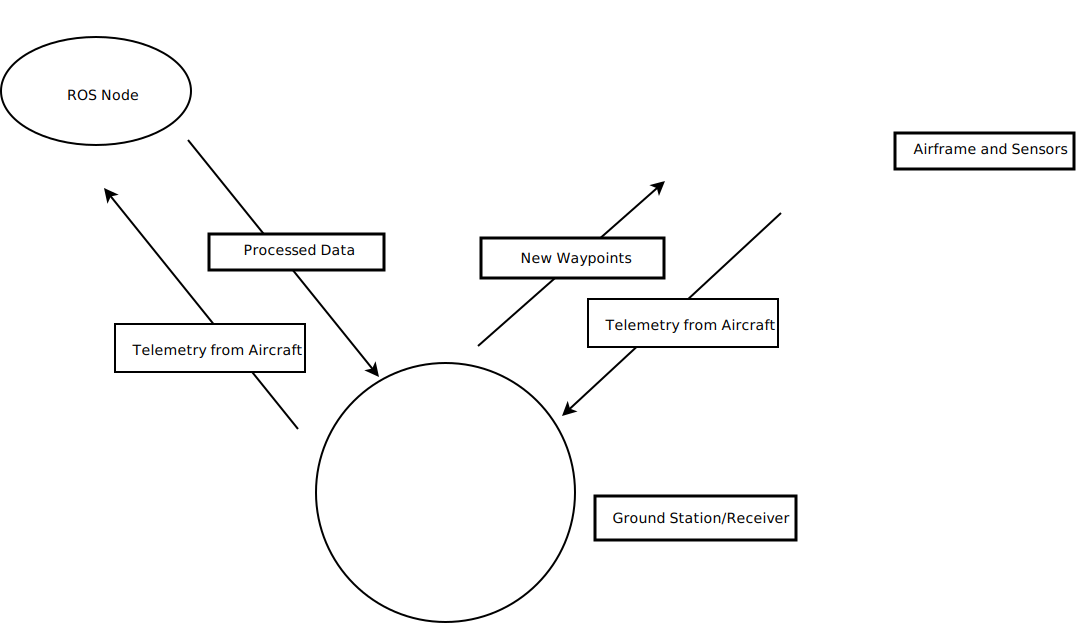
\includegraphics[scale=0.26]{System_Diagram.eps}  
    \caption{Systems diagram, showing the communication structure between aircraft, groundstation, and ROS node}
    \label{system_diagram}
\end{figure}

\section{Message Passing}
Despite the name, ROS is not an operating system but can be thought of more as a highly capabale message-passing interface between different processes, be they sensor outputs or on computer operations such as matrix decomposition. It serves as a way of uniting sensors and platforms from different areas that might have been developed independently. In the case of this project, a package within ROS was used to receive MAVlink messages from the autopilot and effectively unpack them as sensor outputs, with the specific sensors outlined in chapter 2. The format in which ROS does this is by setting up nodes. Nodes can have any number of functions, from receiving data, referred to as "subscribing", sending data, referred to as "publishing", as well as performing intra nodal operations based on ROS packages, such as applying a Kalman filter to data. Publishing data (referred to as a "topic") in ROS allows for other nodes to subscribe to that particular topic. The structure becomes very similar to that of a flow chart, where data may enter one node, and then be published again after the required operations have been performed on it. 

One of the great benefits of ROS is that it allows for nodes to be written in different programming languages, the most prevalent being C++ and Python, making multi-author projects simpler and more effective as each person can write programs in the language they're most comfortable with and still be sure any output can be effectively received by a node in a different language. 

Mavlink extendable communication node for ROS, or MAVROS, was an essential package to the project for a number of reasons. Aside from unpacking MAVLink messages, it had a number of features essential to me as the aircraft operator during the experiment, such as monitoring the current mode of the autopilot, monitoring aircraft voltage and autopilot health, and checking radio link status. Other features allowed for specific commands to be sent to the autopilot from within the created node, such as various waypoint navigation commands. Figure \ref{fig:mavros_rqt_graph} shows the various topics published by the MAVROS node.

\begin{figure}[!ht]
	\centering
	\includegraphics[scale=0.6]{mavros_rqt_graph.png}
	\caption{Graph of various topics published by the MAVROS node}
	\label{fig:mavros_rqt_graph}
\end{figure}

\section{Node Implementation}
While the project relied heavily on matrices, the primary model-building algorithm required a considerable amount of processing time and memory. Besides being compatibile with ROS, C++ allows the user to directly monitor memory usage, which is of particular use if an onboard computer is ever required. As well, C++ and ROS both allow the user access to the Eigen linear algebra and general matrix manipulation library. Despite several shortfalls with regards to aliasing, Eigen performed well as a library, with built-in Cholesky decomposition required in Gaussian process sampling.

\section{Data Visualization}
The primary use for MATLAB in this project was for visualization purposes. A small 2D cone library was created for visualization of the flow fields and feature recognition based on the specific output from the model developed in the ROS C++ node. This made data formatting almost trivial as it allowed me to simply output the uncertainty, magnitude, and direction of each of the vectors from the model and the MATLAB script, with the results in the following chapter.

\chapter{Results} 

\section{Data Collection}

Data was collected in a large experiment that was deemed to adequately demonstrate the potential of the system, similar to that of \cite{Leonard10}. The experiment was performed from June 9th through June 15th, during which time the platform was taken out to Pentland Hills Regional Park, south of Edinburgh.
\begin{figure}[!ht]
	\centering
    \includegraphics[scale=0.15]{in_field_picture.jpg}  
    \caption{Ground station on third day of experiments.}
    \label{fig:in_field}
\end{figure}
The location was chosen based on a very specific set of geological land forms to maximize the chances of viewing these features through the wind mapping process. To do this, there needed to be a feature that was both relatively easy to access, as the experiment needed to last for many days, and be large enough to significantly affect the wind currents in the area. As well, a secondary objective was that it would be located near a flat region so that the data could in effect have a "normalized" region, or one with no features as a side by side comparison, both of which would be expressed in the data and recognizable in the resulting processed data.

To validate that the wind vector readings returned by the aircraft were reasonable, two anemometers (wind speed gauges) were used, one at the top of the nearby feature and one at the ground station. Figure \ref{fig:in_field} shows the basic field infrastructure minus the second anemometer, which is not visible in the picture. The hill in the left portion of the picture acted as the target feature. It was deemed a reasonable choice after hiking to the top as well as doing several test flights to ensure that reality followed the theory regarding wind speed around large features.

\begin{figure}[!ht]
	\centering
	\includegraphics[scale=0.46]{flight_plan_3.png}
	\caption{Flight plan after some tests and variations}
	\label{fig:flight_plan_1}
\end{figure}

Similar to the work in \cite{Leonard10}, the flight path was created before going out to the field utilizing observations based on previous trips to the location and a topographical map and was based primarily on experiment requirements to ensure that wind around the two major features, the flatland and mountain, were measured by the UAV. The flights themselves covered an approximately 50,000 to 70,000 square meter area, limited primarily by radio connection and the aircraft operator line of sight as required by British law for non-commercial UAV applications. As well, due to the limits on battery life, a trial and error method was used such that it became apparent very quickly what the best route in the given conditions were. The initial flight plans allowed the aircraft to fly too far, leading to loss of signal and a repeat of the data, as well as an inability to fly to all of the waypoints. The repetition of data raised the need for added safeguards as repetitive data was still given a unique time stamp suggesting that data was streaming normally. It suggests that future systems will collect and retain more data points with an onboard computer such that signal strength is no longer an issue.

Each flight lasted approximately 20 minutes. Due to the relatively short flight times, it was then considered an independent event. That is, each flight was considered to have taken place instantaneously based on the fact that the wind was observed to change relatively slowly. Possible solutions to this are covered further in the "Future Work" section of chapter 6. 

Of course, the plane can't fly all of the points at once, it takes time to reach them. Instead, the assumption is based on the idea that the weather takes a not insignificant amount of time to change. That is, the wind speed and direction (ie, the parts this paper is primarily concerned with) will not change significantly in the twenty minutes that the plane is flying

The altitude was a very important part of the experiment as I was trying to measure the expected increased wind speed over mountainous features. This made for truly nail-biting experiences as depth perception is effectively non-existent when the aircraft was at significant distances.

Once the data had been collected, it was filtered and placed into a two-dimensional grid for analysis, the algorithms for which are explained further in the next section. The grid choice itself was based on work done by Wani and Yesilbudak \cite{Wani13}, where a relatively coarse grid size gives a more representative appearance to the data, especially since the coarser grid size means more data per grid square. After data collection, I manually adjusted the grid size for the collected data before becoming satisfied with the resulting grid space. In the future work section of chapter 6, I suggest a method by which the grid can be made finer with the use of a multi-rotor platform.

Uncertainty values for the individual boxes were calculated using standard deviation equation
\begin{equation}
	\sigma=\sqrt{\frac{1}{N}\sum\limits_{i=1}^N(x_i-\mu)^2}
	\label{eq:standard_deviation}
\end{equation}
where $N$ is the number of measurements for that particular grid location, $\mu$ is the mean, and $x_i$ represents the individual values in the subset.

Tables \ref{table:1} and \ref{table:2} give a general idea as to the conditions in the field during the experiment.
\begin{table}[!ht]
\begin{center}
	\begin{tabular}{|c| c|}
	\hline
	Date&Weather\\	
	\hline
	June 9&sunny with light breeze from the SW\\
	June 10&sunny with light breeze from the SW\\
	June 11&sparse clouds with light wind from NE\\
	June 12&overcast with moderate wind from NE\\
	June 13&drizzling rain plus moderate wind from NE\\
	June 14&sparse clouds with light wind from NE\\
	June 15&sunny with light breeze from SW\\
	\hline	
	\end{tabular}
\end{center}
\caption{Summary of weather conditions on each of the flying days}
\label{table:1}
\end{table}

\begin{table}[!ht]
\begin{center}
	\begin{tabular}{|c| c| c|}
	\hline
	Date&Number of Flights&Max Wind Speed(mph)\\	
	\hline
	June 9&5&4.3\\
	June 10&4&5.0\\
	June 11&5&15.4\\
	June 12&5&24.6\\
	June 13&1&18.2\\
	June 14&5&11.7\\
	June 15&4&5.2\\
	\hline	
	\end{tabular}
\end{center}
\caption{Maximum wind speeds encountered on each day of flying, with each flight starting on the hour, and each day of experimentation beginning at 11:00}
\label{table:2}
\end{table}

\clearpage
\section{Vector Field Interpolation and Regression}
The following graphs are the result of the vector field interpolation method outlined in chapter 3. The graphs themselves are effectively a cutaway from the defined area in the field. Figure \ref{fig:low_wind_raw} shows the initial measurements taken by the aircraft, where the corners of the graph are effectively GPS coordinates. The tilted image of the flying area seen in \ref{fig:re_flight_plan_1} gives the a better orientation to the reader for the rest of the graphs. As well, figure \ref{fig:topo} is a topographical map of the specific region in which the experiments were held. 

\begin{figure}[!ht]
	\centering
	\includegraphics[scale=0.35, angle = -40]{flight_plan_3.png}
	\caption{Flight plan after some tests and variations}
	\label{fig:re_flight_plan_1}
\end{figure}

\begin{figure}[!ht]
	\centering
	\includegraphics[scale=0.45, angle=-45]{topographical_mod.png}
	\caption{Topographical map of highlighting the feature area}
	\label{fig:topo}
\end{figure}

Figure \ref{fig:low_wind_raw} shows the resulting data from a single flight on the first day of experimentation. Due to the low magnitude and direction, feature recognition was not possible in these conditions. However, knowing the region, I was sure that the wind would pick up and some unique data would be collected. As well, since the plane being pushed off its path by the wind, the uncertainty values are relatively low, with noisy uncertainty based around $5^\circ$, depending on the output from the standard deviation for the particular cell in which the measurements reside.

\begin{figure}[!ht]
	\centering
	\includegraphics[scale=0.2]{low_wind_raw.jpg}
	\caption{Data representative of one flight done four hours into the experiment}
	\label{fig:low_wind_raw}
\end{figure}
The first graph of interpolated data is shown in figure \ref{fig:low_wind_interp}. Again, as far as feature recognition was concerned, no unique patterns emerged from this data as the wind speed was simply too low to pick up any details resulting from a large feature. Due to the nature of the algorithm outlined in chapter 3, a maximum uncertainty of $7^\circ$ was reached. This uncertainty seemed low, but may be a reasonable result as there appeared to be very little variation in speed or direction for this particular flow field. Certainly, as we get into the higher velocity wind fields, the change in uncertainty becomes apparent as well as unique trends in the data.

\begin{figure}[!ht]
	\centering
	\includegraphics[scale=.2]{low_wind_interp2.jpg}
	\caption{interpolation of the low wind field shown in figure \ref{fig:low_wind_raw}} 
	\label{fig:low_wind_interp}
\end{figure}

\begin{figure}[!ht]
	\centering
	\includegraphics[scale=0.2]{Windy_raw.jpg}
	\caption{Flow field from one flight on the fourth day of experiments}
	\label{fig:Windy_raw}
\end{figure}

Figure \ref{fig:Windy_raw} shows the data taken by the plane on the fourth day of flights where the wind reached its maximum. The primary difference to note is that the wind direction has flipped almost exactly $180^\circ$ degrees to what was measured during the first two days. The wind appears to be acting similarly to that of a ball thrown into the air. That is, the change in direction of the wind is accompanied by a zero-velocity point. This is corroborated by weather from a weather station from the nearby town of Penicuik which shows this change of direction in the "Wind Dir" plot at the bottom of figures \ref{fig:curious_weather} and \ref{fig:curious_last_day} which occurred on the morning of the third and sixth days respectively.

Figure \ref{fig:Windy_raw} shows data from the fourth day, or 97 hours into the experiment, which displays quite high wind speeds as noted in table \ref{table:2}, with two flights making up the data displayed in the figure. A timed landing, battery change, software start, and launch took just over five minutes. With higher uncertainty values, likely from the plane being tossed around considerably in the high wind, the data appears to show the start of a warping within the wind map caused by the nearby hill. 

Figure \ref{fig:Windy_interp} shows the interpolated vector field for the windy day, with uncertainty values increasing considerably especially near the higher magnitude areas of the graph in the top left.

\begin{figure}[!ht]
	\centering
	\includegraphics[scale=0.2]{windy_interp_moded.jpg}
	\caption{Interpolation of the windy flow field shown in figure \ref{fig:Windy_raw}}
	\label{fig:Windy_interp}
\end{figure}

Finally, figure \ref{fig:windy_inter_reg_mid} shows a predicted vector field based on the data gathered during the experiment. The values are based on the input locations and time, which in this case is equivalent to 56 hours into the experiment, or between experiments done on days three and four.

\begin{figure}[!ht]
	\centering
%	width = 14cm, height = 5.7cm 
	\includegraphics[scale = 0.2]{windy_inter_reg_mid.jpg}
	\caption{Plot of data predicted at approximately 56 hours into the experiment}
	\label{fig:windy_inter_reg_mid}
\end{figure}

\clearpage
\section{Weather}
The weather of Scotland is difficult to forecast for even the most experience of Scottish weather people, and to do even several week long experiments is likely not enough to create a model that will be accurate a majority of the time. However, I believe that the data shown here shows that there are patterns that an be associated with specific weather types.

One will notice in figures \ref{fig:low_wind_raw} and \ref{fig:Windy_raw} that there is a complete change in wind direction, which is confirmed by the weather graphs taken from a weather station in Penicuik. It was theorized before as well in chapter 2 that the use of the aircraft's barometer might be useful in monitoring oncoming weather.
\begin{figure}[!ht]
	\centering
	\includegraphics[scale=0.63]{curious_weather.png}
	\caption{Weather graphs from the third day of experimentation \cite{wUnderground}}
	\label{fig:curious_weather}
\end{figure}
\begin{figure}[!ht]
	\centering
	\includegraphics[scale=0.63]{last.png}
	\caption{Weather on the final day of experiments, where it was nearly identical to the first two days of flying \cite{wUnderground}}
	\label{fig:curious_last_day}
\end{figure}
Not only that, but in figure \ref{fig:pressure_compare} the graphs depict similar results to each other, indicating the oncoming storm. However, should an aircraft stay aloft for a long enough period of time, it would require a distance sensor to measure the distance between itself and the ground to get an accurate reading for pressure, and to safely stay aloft if there is either no terrain following option available or it is simply not being used, or there is insufficient GPS coverage.
\begin{figure}[!ht]
	\centering
	\includegraphics[scale=0.2]{Pressure_from_AP.jpg}
	\caption{Comparison of pressures: the top graph is from a local weather station, the bottom is from the autopilot on takeoff}
	\label{fig:pressure_compare}
\end{figure}


\clearpage
\section{Feature Recognition}
For the area investigated, feature detection varied according to wind direction and magnitude. Early experiment wind readings, shown in figure \ref{fig:low_wind_interp}, blew towards the ground station and the mountains behind. Once the direction changed and the wind speed increased, as shown in figure \ref{fig:Windy_interp}, the algorithm was able to discern features based on changes in wind speed magnitude over the field, with results in figures \ref{fig:k_means} and \ref{fig:final_cluster} 
\begin{figure}[!ht]
	\includegraphics[scale=0.2]{surface_mag.jpg}
	\caption{An example from the feature recognition algorithm}
	\label{fig:k_means}
\end{figure}
\begin{figure}[!ht]
	\includegraphics[scale=0.2]{clustered_cells.jpg}
	\caption{End result of the k-means clustering, showing the values associated with the feature}
	\label{fig:final_cluster}
\end{figure}
Figure \ref{fig:k_means} effectively tracks the movement of one of the centroids during the algorithm run time, where the lighter areas signify movement towards convergence. Figure \ref{fig:final_cluster} shows the resulting data taken from the previous graph and isolated into the two clusters.The primary cluster of interest, shown in blue, in fact represents the flight locations over the feature of interest. When visually compared with the actual flight and topological maps, the middle of the cluster appears to be offset from the feature, which might be due to windspeed remaining high even after passing the feature.

\chapter{Conclusion and Future Work}
\section{Conclusion}
For this project, I set out to create a system based on a UAV platform that would incorporate aspects of machine learning allowing it to map the wind flow over a particular region and create a model based on that data to create maps for the times during which the aircraft was not flying. It was found that the system was easy transported and allowed for a relatively wide area for remote sensing when compared with the typical wind mast deployment method mentioned in chapter 1, suggesting that it is a superior method for wind mapping over a large area.  

I took the project from inception, to the physical stage by familiarizing myself with a new platform, the radian pro, and performing initial flights to understand its handling characteristics in the event of a fault in the field with the autopilot on board. I then adapted an autopilot board and sensors to an aircraft not designed for such equipment through airframe modification and 3D printed CAD models. I continued on to learn MAVROS and how to network the aircraft with a ROS node and send commands from within that ROS node to the aircraft. All the while, I became familiar with numerous machine learning processes before focusing on Gaussian processes as the method of data interpolation and regression. I then utilized a $k$-means clustering algorithm to identify features in the area. Besides machine learning, I became familiar with weather movements, in Scotland no less, which is no small feat, and compared my resulting data with data from a nearby weather stations, showing reasonable similarity between the two with the intent of future development in creating models for weather prediction.

The UAV then is a prime candidate for future development within the areas of pollution tracking and broader weather mapping. I have shown that it is a platform that, when equipped with the appropriate software, can be an effective measurement tool itself. This is opposed to the more generally held view of utilizing the UAV as visual aid or as the manoeuvres of the UAV being the topic of interest.

\section{Future Work}
There are a number of steps that can be taken to further improve upon this work, from increasing the endurance or range of the aircraft, to making it more self contained through the use of an onboard computer. As well, there are several applications and scenarios for which it would be useful in testing.

A relatively easy addition would be that of an onboard computer. While I have personal experience with autopilot-onboard computer communications, to ensure a reliable as possible platform, it was not included in the design. In the future, it would be useful for onboard model creation as data transfer would also be much more reliable, though computing power would likely suffer as well as aircraft endurance.

One issue I continually battled was that of flight time in a dynamic environment. While many hobby pilots are "fair weather flyers", I had the challenge of flying in winds up to 11m/s which proved to be a greater strain on the batteries than I had anticipated. There is considerable work in the field of long endurance aircraft such as that pictured in figure \ref{fig:taleaus} currently in development by the United States Navy, utilizing both thermal-seeking flying techniques and solar technology to remain aloft for long periods of time.
\begin{figure}[!ht]
	\centering
	\includegraphics[scale=0.2]{taleaus.jpg}
	\caption{The first three iterations of the TActical Long Endurance Unmanned Aerial System developed by the US Navy TALEUAS \cite{Vogt}}
	\label{fig:taleaus}
\end{figure}
This would allow for both longer and larger area of coverage, though the generated map could have discrepancies between regions as the times would start to vary significantly between measurements. This leads to another future development: multi agent flight systems.

There is currently a large amount of research being done on aircraft swarms as well. One of which, shown in figure \ref{fig:plane_swarm}, has flown 30 aircraft at once to date utilizing an open source mesh grid protocol. With that system, it would be reasonable to have multiple agents collecting data at once over a large area and creating a joint model thanks to the mesh network. If combined with my description of the high endurance aircraft mentioned in the previous paragraph, the system could possibly be a persistent monitoring system covering a large area almost at once.

If finer resolution is a requirement in the future, another development would take the form of a multirotor with a stabilized boom holding one or more air speed sensors to sample at a continuous step. The finer resolution can be attained as the multirotor can hover and move incrementally. However, range will suffer greatly as the relationship between resolution and area coverage is an inverse relationship for a fixed amount of time.

Having live in the region in which the experiment was done, it is clear that a number of models would need to be created to adequately predict weather based on specific conditions. While the patterns discovered in this project appeared fairly well defined, I hypothesize that there are a number of models that describe individual categories of weather systems, suggesting that many experiments are required to gather data, then a classification run on the resulting models to predict which particular type of system might be in the area, or the probability of a particular system arriving in the near future. 

Certainly, there is no shortage of directions in which this project could develop, but rather the difficulty comes in choosing the correct direction.

\begin{thebibliography}{10}%Any two digit number for more than nine references

\bibitem{Anderson01}
	Anderson, Jr., J.D. (2001). \emph{Fundamentals of Aerodynamics} McGraw Hill

\bibitem{Ariff11}
	Ariff, O.K. and Go, T.H. (2011). \emph{Waypoint Navigation of Small-Scale UAV incorporating Dynamic Soaring} The Journal of Navigation

\bibitem{Bailey97}
	Bailey, B.H., McDonald, S.L., Bernadett, D.W., Markus, M.J. and Elsholz, K.V. (1997). \emph{Wind Resource Assessment Handbook} National Renewable Energy Laboratory

\bibitem{Barthelmie14}
	Barthelmie, R.J., Crippa, P., Wang, H., Smith, C.M., Krishnamurthy, R., Choukulkar, A., Calhoun, R. et al (2014). \emph{3D Wind and Turbulence Characteristics of the Atmospheric Boundary Layer} American Meteorlogical Society

\bibitem{Bohling05}
	Bohling, Geoff (2005). \emph{Kriging},
http://people.ku.edu/~gbohling/cpe940/ Kriging.pdf
	
\bibitem{Bretherton75}
	Bretherton, F.P., Davis, R.E., and Fandry, C.B. (1975). \emph{A technique for objective analysis and design of oceanographic experiments applied to MODE-73} Deep-Sea Research
	
\bibitem{Brezoescu13}
	Brezoescu, A., Castillo, P. and Lozano, R. (2013). \emph{Wind estimation for accurate airplane path following applications} International Conference on Unmanned Aircraft Systems	
	
\bibitem{Cully15}
	Cully, A., Clune, J., Tarapore, D., and Mouret, J. (2015). \emph{Robots that can adapt like animals} Nature	
	
\bibitem{Duda01}
	Duda, R.O., Hart, P.E. and Stork, D.G. (2001). \emph{Pattern Classification: Second Edition} Wiley-Interscience
	
\bibitem{Duvenaud14}
	Duvenaud, D.K. (2014). \emph{Automatic Model Construction with Gaussian Processes} University of Cambridge, Pembroke College

\bibitem{Gorman08}
	Gorman, R.M. (2008). \emph{Intercomparison of Methods for the Temporal Interpolation of Synoptic Wind Fields} Journal of Atmospheric and Oceanic Technology
	
\bibitem{Hemakumara13}
	Hemakumara, P. and Sukkarieh, S. (2013). \emph{Learning UAV Stability and Control Derivatives Using Gaussian Processes} IEEE Transaction on Robotics

\bibitem{Kan13}
	Kan, E.M., Lim, M.H., Ong, Y.S., Tan, A.H. and Yeo, S.P. \emph{Extreme learning machine terrain-based navigation for unmanned aerial vehicles} Neural Computation and Applications

\bibitem{Kothari14}
	Kothari, M., Postlethwaite, I. and Gu, D. (2014). \emph{UAV Path Following in Windy Urban Environments} Journal of Intelligent Robotic Systems

\bibitem{Krause10}
	Krause, A. (2010) \emph{Advanced Topics in Machine Learning} Lecture given at Caltech for CS/EE 253, Feb 24, 2010

\bibitem{Kuroki09}
	Kuroki, Y., Young, G.S. and Haupt, S.E. (2009). \emph{UAV navigation by an expert system for contaminant mapping with a genetic algorithm} Expert Systems with Applications

\bibitem{Lega10}
	Lega, M. and Napoli, R.M.A. (2010) \emph{Aerial infrared thermography in the surface waters contamination monitoring} Desalination and Water Treatment

\bibitem{Leidwanger13}
	Leidwanger, J. (2013). \emph{Modeling distance with time in ancient Mediterranean seafaring: a GIS application for the interpretation of maritime connectivity} Journal of Archaeological Science

\bibitem{Leonard10}
	Leonard, N.E., Paley, D.A., Davis, R.E., Fratantoni, D.M., Lekien, F. and Zhang, F. (2010) \emph{Coordinated Control of an Underwater Glider Fleet in an Adaptive Ocean Sampling Field Experiment in Monterey Bay} Journal of Field Robotics
	 
\bibitem{Liu13}
	Liu, B., Luo, X. and Wei, H. (2013). \emph{Research on the Method of Wind Speed Interpolation: Based on Spaitally Anisotropic Analysis} International Conference on Mechatronic Sciences, Electrical Engineering, and Computer Engineering

\bibitem{Nelson07}
	Nelson, D.R., Barber, D.B., McLain, T.W. and Beard, R.W. (2007). \emph{Vector Field Path Following for Miniature Air Vehicles} IEEE Transactions on Robotics

\bibitem{NOAA15} 
	NOAA \emph{Numeric Weather Prediction} https://www.ncdc.noaa.gov/data-access/model-data/model-datasets/numerical-weather-prediction

\bibitem{Parasuraman09}
	Parasuraman, R., Cosenzo, K.A. and De Visser, E. (2009) \emph{Adaptive Automation for Human Supervision of Multiple Uninhabited Vehicles: Effects on Change Detection, Situation Awareness, and Mental Workload} Military Psychology

\bibitem{Peacock13}
	Peacock, T. and Haller, G. (2013) \emph{Lagrangian coherent structures: The hidden skeleton of fluid flows} Physics Today

\bibitem{Rasmussen96}
	Rasmussen, C.E. (1996) \emph{Evaluation of Gaussian Processes and Other Methods for Non-Linear Regression} Graduate Department of Computer Science, University of Toronto

\bibitem{Rasmussen06}
	Rasmussen, C. E. and Williams, C. K. I. (2006) \emph{Gaussian Processes for Machine Learning} MIT Press
	
\bibitem{Saljic12}
	Saljic, N. (2012) \emph{Majestic Matterhorn Portraits by Nenad Saljic} from \texttt{www.mymodernmet.com/profiles/blogs/nenad-saljic-matterhorn-portraits}
	
\bibitem{Shie13}
	Shie, R. and Chan, C. (2013). \emph{Tracking hazardous air pollutants from a refinery fire by applying on-line and off-line air monitoring and back trajectory modeling} Journal of Hazardous Materials	
	
\bibitem{Smidl12}
	Smidl, V. and Hofman, R. (2012). \emph{Navigation of UAVs for Tracking of Atmospheric Release of Radiation} 51st IEEE Conference on Decision and Control	
	
\bibitem{StachnissX}
	Stachniss, C., Plagemann, C., and Lilienthal, A.J. (X). \emph{Learning Gas Distribution Models using Sparse Gaussian Process Mixtures} Autonomous Robots
	
\bibitem{Vogt}
	Vogt, C [photograph] (Private collection)

\bibitem{Wani13}
	Wani, M.A. and Yesilbudak, M. (2013). \emph{Recognition of Wind Speed Patterns Using Multi-Scale Subspace Grids with Decision Trees} International Journal of Renewable Energy Research

\bibitem{windMonitor}
\emph{Complete Solutions for Small Wind Turbine Site Assessment} \texttt{windmonitoring.com}

\bibitem{wUnderground}
\emph{Historical Weather} \texttt{www.wunderground.com/history}

\end{thebibliography}

\end{document}